% !TEX encoding = UTF-8 Unicode
%!TEX root = ../Main/thesis.tex
% !TEX spellcheck = en-US
%%=========================================
\documentclass[../Main/thesis.tex]{subfiles}
\begin{document}
\chapter[Hilbert Huang transform for high frequency pulse detection]{Hilbert Huang transform for high frequency pulse detection}
\label{sec:hht}

Most signal analysis methods such as Fourier transform, impose an a-priory basis function on the signal to be analyzed. In the case of Fourier analysis, the basis functions are trigonometric extensions. Although this implies a rigorous mathematical treatment, the resulting signal decomposition is limited by the mathematical assumptions. Two such assumptions are linearity and stationarity. As most phenomena in nature are non linear and non stationary, this mathematical approach, although rigorous, lacks an important property: Adaptivity. The latter refers to capturing the intrinsic properties of a signal, without imposing an a-priory basis function, \cite{huang98}, \cite{huang08}. 
\justify 
The Hilbert Huang transform (HHT) was precisely developed to deal with non linear and non stationary processes, in an adaptive fashion. It combines Hilbert spectral analysis with the so call empirical mode decomposition (EMD), to adaptively decompose a signal into its fundamental components called intrinsic mode functions (IMF), \cite{huang98}.
The EMD is the pillar of the Hilbert Huang transform, and we shall describe it in detail shortly. The richness of the HHT span from the analysis of differential equations, to the study of geophysical phenomena, and by no means restricted to the former and the latter. It has been successful applied to the analysis of solutions of nonlinear differential equations such as the Duffing and the Lorentz equations. The intrinsic frequency, the forcing function and the low intensity subharmonics of the numerical solutions for the nonlinear Duffing equation has been extracted through the EMD process, \cite{huang98}. The decomposition of the solutions of Lorentz equation, revealed \say{transient components with different frequencies and damping characteristics}, which agreed with previous studies, \cite{huang98}. Its application to seismic wave propagation, made it possible to identified high and low frequency seismic wave [Vasudevan and Cook 2000, Zhan et al, 2003a, 3003b, zhang 2000]. In particular, its decomposition of the seismic waves induced by the 1999 Taiwan earthquake, which caused tremendous human and material lost,  revealed that the Fourier transform underestimated low frequency energy due to its linear characteristics [Huang et al 2001]. 
\justify
The Hilbert Huang transform emerged as a general signal decomposition tool, and can in principle and in theory be applied to any signals. To further show its potential, in this chapter we apply the HHT to bearing fault analysis. Section \ref{sec:emd}, presents the empirical mode decomposition (EMD), which is the back bone in decomposing a signal adaptively. In section \ref{sec:pulse}, we begin by showing that the HHT, coupled with a robust seasonal decomposition method, is able to recover the high frequency pulses emitted by a bearing with a crack. As emphasized in the greeks mythology, any hero has an Achilles hill, and the HHT is no exception from this rule. Therefore in closing, we outline some of the limitations of the HHT based on the empirical mode decomposition.
\justify
\section{Hilbert spectral analysis and the empirical mode decomposition}
\label{sec:emd}
As any new methods, the Hilbert Huang transform strives in improving upon previous signal processing paradigms. It rests on adaptivity, non linearity, non stationarity and physical meaningful time-frequency-energy paradigm. The latter is akin to the fundamental concept of uniqueness in the study of the solution of differential equations.
[Transition]. 
In Fourier analysis, given a time dependent signal $S(t)$, we can express it as the following complex expansion
\begin{equation} \label{eq:fourier}
S(t) = \sum_{j=1}^{\infty}a_{j}\exp(i\omega_{j}t),
\end{equation}
where $a_{j}, \omega_{j}$ are constant amplitudes and frequencies respectively, and $i = \sqrt{-1}$. The Hilbert Huang transform generalizes the Fourier expansion (\ref{eq:fourier}) with time dependent amplitude $a(t)$ and frequency $\omega(t)$ as 
\begin{equation} \label{eq:hht}
S(t) = \sum_{j=1}^{n}a_{j}(t)\exp\left(i\int \omega_{j}(t)\mathrm{dt}\right).
\end{equation}
Equation (\ref{eq:hht}) expresses non stationarity as opposed to equation (\ref{eq:fourier}), by providing amplitude and frequency modulation. Here amplitude and frequency modulation refers to the time dependent amplitude $a(t)$ and frequency $\omega(t)$. This is where Hilbert transform comes into play. The Hilbert transform denoted by $H(t)$ of the signal $S(t)$ is given by
\begin{equation}\label{eq:hilbert}
H(t) = \frac{P}{\pi}\int_{-\infty}^{\infty}\frac{S(\tau)}{t-\tau}\mathrm{d\tau},
\end{equation}
where $P$ is the Cauchy principal value of the singular integral \cite{huang08}. The amplitude $a(t)$ and the frequency $\omega(t)$
can hence be deduced by 
\begin{equation}\label{eq:amplitude}
a(t) = \sqrt{S(t)^{2} + H(t)^{2}}
\end{equation}

\begin{equation}\label{eq:frequency}
\omega(t) = \frac{d}{dt}\left(\tan^{-1}\left(\frac{H(t)}{S(t)} \right) \right)
\end{equation}
The amplitude and frequency modulation obtained from Hilbert transform in equation (\ref{eq:amplitude}, \ref{eq:frequency}) does not always provide a meaningful physical description of a signal \cite{huang98}, \cite{huang08}. The empirical mode decomposition (EMD), decomposes a given signal, such that the resulting subcomponents gives physically meaningful amplitude and frequency modulation, \cite{huang98}. For a given signal $S(t)$, the objective is to obtained its $n$ fundamental parts $s_{j}, j =1,\cdots,n$, called intrinsic mode functions (IMF), through the empirical mode decomposition, such that
\begin{equation}\label{eq:emd-decomposition}
S(t) = \sum_{j=1}^{n}s_{j}(t) + r(t),
\end{equation}
where $r(t)$ is the residual, which is either a constant or a monotone function. The obtention of the intrinsic mode functions $s_{j}$, by means of the empirical mode decomposition, relies on the following key assumptions.
\begin{definition}\label{def:emd}
An intrinsic mode function (IMF) must satisfy the following conditions:
\begin{enumerate}
\item The number of extrema and the number of zero crossing must either equal or differ by one 
\item At any data point, the mean value of the envelope defined using the local maxima and the envelope defined by using the local minima is zero.
\end{enumerate}
\end{definition}
The empirical mode decomposition is an iterative algorithm that generates intrinsic mode functions, each satisfying definition \ref{def:emd}.
For an input signal $S(t)$, the first step in to compute the upper and the lower envelope $u(t)$ and $l(t)$, followed by computing the mean $m(t)$ between the upper and the lower envelop. In the next step, the difference between the signal $S(t)$ and $m(t)$ is computed and is given the name proto intrinsic mode function (IMF): h(t) = $S(t)-m(t)$.
The proto-IMF is a real IMF if it satisfies the following stoping criteria \cite{huang08}:
\begin{stoppage criterion}\label{cr:stoppage}
The number of zero crossing and extrema equal or at most differ by one after 3 or 8 consecutive iterations
\end{stoppage criterion}
In the stoppage criterion \ref{cr:stoppage}, a zero crossing is the point where a function changes sign. If it does not satisfy the above criteria, further processing is done. The whole process can be summarize in the following pseudo algorithm:
 %The empirical mode decomposition can be sum up in the following algorithm
\begin{algorithm}
  \begin{algorithmic}[1]
    \STATE Step 1: input signal $S(t)$
    \STATE Step 2: Compute $u(t)$, $l(t)$ and $m(t) = mean(u(t), l(t))$
    \STATE Step 3: Compute the proto IMP $h(t) = S(t) - m(t)$
    \STATE Step 4: Check if stoppage criterion \ref{cr:stoppage} is satisfied. If it is go to next step, if not
    set $S(t) = h(t)$ and start from step 2
      \STATE Step 5: h(t) = c(t) where c(t) is an IMF. Set r(t) = S(t)-c(t), where r(t) is the residual between the original signal and the IMF.
      if r(t) is monotone or constant you are done. If not set S(t) = h(t) and start from step 1 to compute the next IMF
  \end{algorithmic}
\end{algorithm}
%The departure of the HHT from the well known signal analysis tool such as Fourier analysis, can be sum up in the following statements: 
\begin{figure}[H] %  figure placement: here, top, bottom, or page
   \centering
   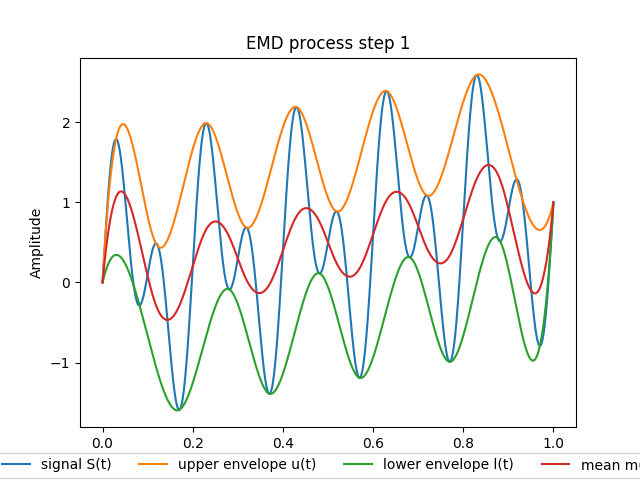
\includegraphics[width=6in]{../fig/emd.png} 
   \caption{The EMD first step. The upper envelope $u(t)$, the lower envelope $l(t)$ of the signal $S(t)$ and the mean $m(t)$ between the upper and the lower envelope are computed in this step}
   \label{fig:emd}
\end{figure}
Figure \ref{fig:emd} describe the first step in the EMD. It shows the original signal $S(t)$, the upper envelope $u(t)$, the lower envelop $l(t)$ and the mean between the upper and the lower envelope. If Figure \ref{fig:emd2}, the difference between the mean $h(t) = S(t)-m(t)$ is shown, while Figure \ref{fig:emd3} shows all the intrinsic mode functions recover from the EMD. As can be seen, the EMD is able to extract the two component of the original signal. The original signal can now be recover by setting 
\begin{equation}\label{eq:recover1}
S(t) = \sum_{j=0}^{2} c_{j}(t) + r(t)
\end{equation}
where $c_{j}$ are the IMFs and r is the residual. Note that the IMFs where derived without an a-priory basis function. This makes the EMD adaptive and able to deal appropriately with non stationary and non linear signals.
\begin{figure}[H] %  figure placement: here, top, bottom, or page
   \centering
   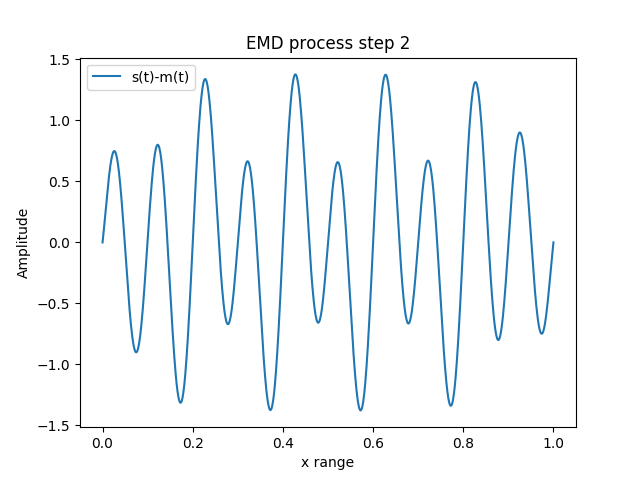
\includegraphics[width=6in]{../fig/emd2.png} 
   \caption{Resulting proto IMF $h(t) = S(t)-m(t)$}
   \label{fig:emd2}
\end{figure}
\begin{figure}[H] %  figure placement: here, top, bottom, or page
   \centering
   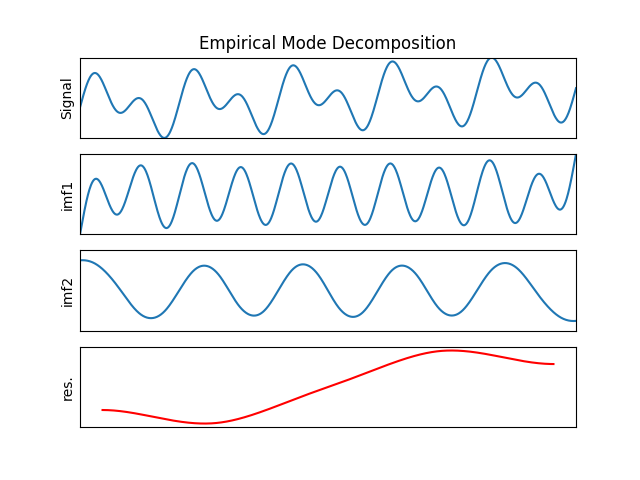
\includegraphics[width=6in]{../fig/imfEMD.png} 
   \caption{The intrinsic mode functions (IMF ) and the residual (in red) generated from the input signal $S(t) = \sin(10 \pi t) + \sin(20 \pi t) $}
   \label{fig:emd3}
\end{figure}
\justify
The intrinsic mode functions obtained through the EMD process constitute an adaptive basis that satisfies the mathematical properties of convergence, completeness, orthogonality and uniqueness, \cite{huang98}. Furthermore, if $a_{j}(t)$ and $\omega_{j}(t)$ are amplitude and frequency modulation corresponding to IMF $j$, then the original signal $S(t)$ can also be recover as 
\begin{equation}\label{eq:recover2}
S(t) = \Re{\left( \sum_{j=1}^{n}a_{j}(t)\exp\left(i\int\omega_{j}(t)\mathrm{dt}\right)  \right)},
\end{equation} 
where the symbol $\Re(\cdot)$ represents the real part of the expression its encompasses, $i=\sqrt{-1}$, and $n$ is the total number of IMFs obtained from decomposition a signal $S(t)$. Recall that the amplitudes $a_{j}(t)$ and the frequencies $\omega_{j}(t)$ can be computed through the Hilbert transform from equations (\ref{eq:hilbert}, \ref{eq:amplitude}, and \ref{eq:frequency}). An analog representation of equation (\ref{eq:recover2}) in terms of Fourier expansion would be 
\begin{equation}\label{eq:recoverFourier}
S(t) = \Re{\left( \sum_{j=1}^{n}a_{j}\exp\left(i\omega_{j}\right)  \right)},
\end{equation} 
where this time, the amplitude $a_{j}$ and the frequency $\omega_{j}$ are constant. The Hilbert Huang transform (HHT) offers two different approaches to recover a decomposed signal. The first one is described by equation (\ref{eq:recover1}) and include the IMFs, while the second approach is given by equation (\ref{eq:recover2}) and includes the instantaneous amplitude and the instantaneous frequency. This gives the HHT a leverage over Fourier transform in nonlinear an non stationary data analysis.
%%%%%%%%%%%%%%%%%%%%%%%%%%%%%%%%%%%%%%%%%%%%%%%%%%%%%%%%%%%%%%%%%%%%%%%%%%%%%%%%%%%%%
%%%%%%%%%%%%%%%%%%%%%%%%%%%%%%%%%%%%%%%%%%%%%%%%%%%%%%%%%%%%%%%%%%%%%%%%%%%%%%%%%%%%%
%%%%%%%%%%%%%%%%%%%%%%%%%%%%%%%%%%%%%%%%%%%%%%%%%%%%%%%%%%%%%%%%%%%%%%%%%%%%%%%%%%%%%

\section{Application of the Empirical mode decomposition to pulse detection}
\label{sec:pulse}
After introducing the Hilbert Huang transform in the previous section, we are now ready to apply the empirical mode decomposition to a case study: Detecting pulses emitted by a bearing with crack in the outer ring. First of all, a few recalls: Figure \ref{fig:bearing-architecture} shows a geometry of a bearing, with different parts.
\begin{figure}[H] %  figure placement: here, top, bottom, or page
   \centering
   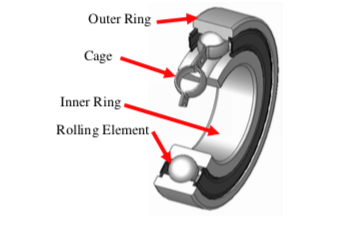
\includegraphics[width=4in]{../fig/bearing.png} 
   \caption{Geometrical representation of a bearing}
   \label{fig:bearing-architecture}
\end{figure}
\justify
A fault occurring at the outer ring is called a ball pass frequency outer ring (BPFO) defect. The frequency (in Hz) at which it occurs can be approximated as followed:
\begin{equation}
BPFO = \frac{np}{2}S\left(1-\frac{BD}{PD}\cos\left(\beta\right)  \right) \nonumber,
\end{equation}
where S is the rotating speed of the motor on which the bearing is attached. nb is the number of rolling elements (balls), BD is a rolling element diameter. The pitch diameter PD is half the hight of the inner ring, and the contact angle $\beta$ is the angle formed when a rolling element touches the cage. The data and the experimental setup used for this case study were described in chapter 2. In this experiment, four bearings are mounted on a motor rotating at 2000 rotations per minutes. The motor runes until bearing number 1 was severely affected by a ball pass frequency outer race defect. The data consists of 984 samples. Each sample contains  acceleration measurements consisted of 20 480 data points, obtained by mounting an accelerometer on each bearing. Recall that an accelerometer is a sensor used to quantify acceleration when a system vibrates. After this background information, let describe the methodology used to detect pulses emitted by a bearing with cracks in the outer ring.
\justify
The method consists of applying the empirical mode decomposition, followed by a robust seasonal trend decomposition method called STL, which stands for Seasonal Trend decomposition procedure based on LOESS,  \cite{Cleveland-et-al-1990}. LOESS is the abbreviation of Locally Estimated Scatterplot Smoother, and is a nonparametric curve fitting procedure. It can be used for \say{Data exploration, diagnostic checking of parametric models and provides a nonparametric regression surface}, \cite{Cleveland-1979}, \cite{Cleveland-et-al-1988}.
\justify
\subsection{Seasonal Trend decomposition based on Loess (STL)}
The STL sequentially applies the locally estimated scatterplot smoother (LOESS) in order to obtain cyclical and trend components of a signal. Here a cyclical component is a periodically occurring pattern in a signal.
If $S(t)$ is a signal, the goal is to obtain the decomposition 
\begin{equation}
S(t) = T(t) + C(t) + R(t),
\end{equation} 
where $T(t)$ an $C(t)$ are the trend and cyclical components, and $R(t)$ is the residual obtained from subtracting  the trend and the cyclical component from the signal. The key ingredient in the STL, is the locally estimated scatterplot smoother procedure. The latter being a non parametric regression method, does not rely on any a-priory assumption on the shape of the curve that needs to be fitted. It therefore provides a flexible approach to curve fitting, by capturing local, as well as global characteristics of a signal. Since pulses emitted by a bearing roller elements passing a crack, are local periodic events on a global scale, the STL provides the necessary mathematical apparatus to capture them.
\justify
By design, the STL is computational efficient, robust in the sense that it uses a robust statistical estimator, and deals very well with missing and distorted data points, \cite{Cleveland-et-al-1990}. In the subsequent paragraphs, an account of the LOESS procedure is presented, followed by the description of the STL method.
\justify
Given a signal represented by a set of $n$ points, conveniently expressed by their coordinates
\begin{equation}
\{ (t_{j}, y_{j}), \quad j = 1, \cdots, n\},
\end{equation}
where $t_{j}$ is the independent variable on the time scale and $y_{j}$ is the dependent variable. The LOESS procedure finds a smooth function $\hat{g}(t)$, defined everywhere on the scale of the independent variable, such that the estimate of $y_{j}$ denoted by $\hat{y}_{j}$ at $t_{j}$ is computed as 
\begin{equation}
\begin{split}
\hat{y}_{j} &= \hat{g}(t_{j}) \\
                &=\sum_{k=0}^{d}\hat{\alpha}_{k}(t_{j})t_{j}^{k}
\end{split}
\end{equation}
where the $\hat{\alpha}_{k}(t_{j})$ are the values $\alpha_{k}$ that minimize 
\begin{equation}
\sum_{k=1}^{n}w_{k}(t_{j})\left(y_{k}-\alpha_{0}-\alpha_{1}t_{k}-\cdots -\alpha_{d}t_{k}^{d}\right)^{2}
\end{equation}
with 
\begin{equation}
w_{k}(t_{j}) = W\left( \frac{t_{k}-t_{j}}{h_{j}} \right)
\end{equation}

\begin{equation}
W(t) = 
  \begin{cases}
  \left(1-t^{3}\right)^{3} &\quad\text{for } 0\leq t \le 1\\
   \0 &\quad\text{for} t\geq 1
 \end{cases}
\end{equation}
and $h_{j}$ is the distance from $t_{j}$ to the nearest neighbor of $t_{j}$. For a signal $S(t)$, by setting 
\begin{equation}
S(t) = T(t) + C(t) + R(t), \nonumber
\end{equation}  
and by applying sequentially the LOESS procedure, the STL is able to extract the trend $T(t)$ and the cyclical component $C(t)$. A detail treatment on how the trend and cyclical components are extracted can be found in  \cite{Cleveland-et-al-1990}.




%%%%%%%%%%%%%%%%%%%%%%%%%%%%%%%%%%%%%%%%%%%%%%%%%%%%%%%%%%%%%%%%%%%%%%%%%%%%%%%%%%%%%%%%%%%%%%
%%%%%%%%%%%%%%%%%%%%%%%%%%%%%%%%%%%%%%%%%%%%%%%%%%%%%%%%%%%%%%%%%%%%%%%%%%%%%%%%%%%%%%%%%%%%%%

\subsection{Results from applying empirical mode decomposition and seasonal trend decomposition base on Loess}
In this section we apply the empirical mode decomposition followed by the seasonal trend decomposition based on LOESS to extract pulses emitted by a failed bearing.
Figure \ref{fig:pulse} shows a flow diagram, describing the methodology to obtain pulses emitted from a bearing with ball pass frequency outer race defect. An input signal goes through the empirical mode decomposition to generate intrinsic mode functions. Furthermore, the STL is applied on the intrinsic mode functions to generate the pulses. 
The outer race ball pass frequency defect, can be viewed as a crack located at the outer ring of a bearing. As the bearings roller elements or balls pass the crack, we should expect to see periodic high frequency pulses in the signal. 

%
\begin{figure}[H]
\begin{tikzpicture}
  [node distance=.8cm,
  start chain=going below,]
     \node[punktchain, join] (intro) {\textcolor{blue}{Signal}};
     \node[punktchain, join] (probf)      {\textcolor{violet}{EMD}};
     \node[punktchain, join] (investeringer)      {\textcolor{blue}{IMFs}};
     \node[punktchain, join] (perfekt) {\textcolor{violet}{STL}};
     %\node[punktchain, join, ] (emperi) {Fast Fourier transform};
     % \node (asym) [punktchain ]  {Asymmetrisk information};
      \begin{scope}[start branch=venstre,
        %We need to redefine the join-style to have the -> turn out right
        every join/.style={->, thick, shorten <=1pt}, ]
        \node[punktchain, on chain=going left, join=by {->}] (risiko) {\textcolor{blue}{Pulse}};
      \end{scope}
      \begin{scope}[start branch=hoejre,]
      %\node (finans) [punktchain, on chain=going right] {Det finansielle system};
    \end{scope}
    \end{tikzpicture}
  \caption{Schematic description of the methodology to obtain pulses which are high periodic high frequency pattern.}
   \label{fig:pulse}
\end{figure}
\begin{figure}[H] %  figure placement: here, top, bottom, or page
   \centering
   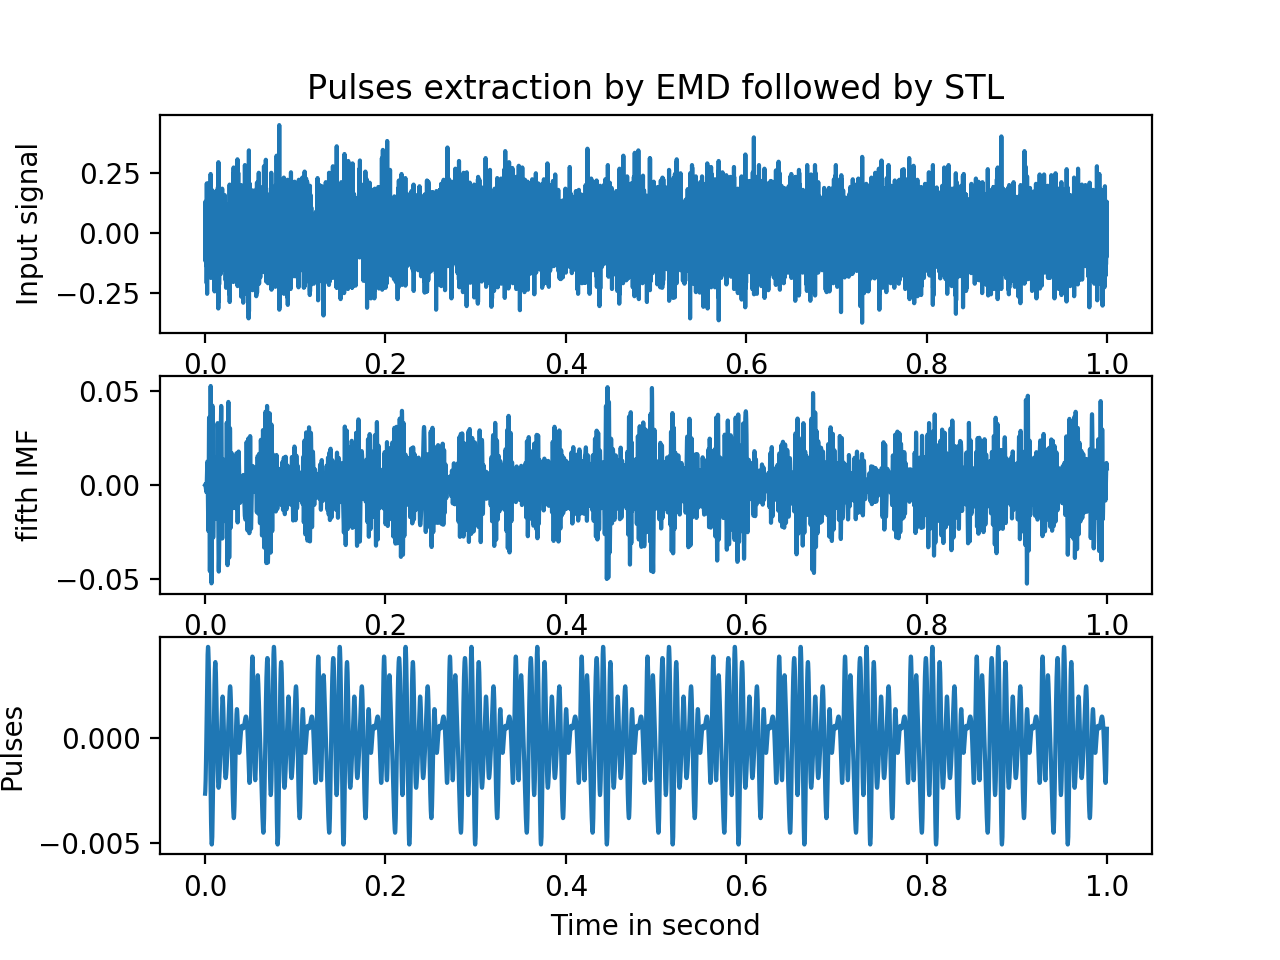
\includegraphics[width=6in]{../fig/emd-stl.png} 
   \caption{Pulses extracted by applying EMD followed by STL. The pulses represent the periodic high frequency pattern emitted by a bearing when the roller elements pass a crack located in the outer ring.}
   \label{fig:emd-stl}
\end{figure}
\justify
Figure \ref{fig:emd-stl} shows, the result from applying the EMD and the STL to an input signal. The top graph represents the input vibration signal obtained by mounting an accelerometer on the defected bearing. The signal is measured after 6020 minutes from the start of the experiment. Recall that, after 9840 minutes, the defect endured by the bearing becomes severe, and the experiment is stoped. The middle graph of Figure \ref{fig:emd-stl} shows the fifth IMF obtained from applying the EMD to the input signal. The IMF exhibits the presence of high frequency patterns. However, it is hard to clearly  identify periodic high frequency patterns. Thats where the STL comes to the rescue. It extracts the periodic high frequency pulses from the IMF with elegance and they can be seen in the bottom graph of Figure \ref{fig:emd-stl}. When a bearing roller element hits the crack, this event can conceptually be interpreted as the generation of a huge amount of energy in a small amount of time, that slowly dies out. The bottom graph of Figure \ref{fig:emd-stl} clearly shows such event. More interprestitit



%The middle graph shows the fifth intrinsic mode function generated from applying the EMD on the input signal. This IMF shows patterns.
%This is precisely what is require to capture a pulse, which can be viewed as a periodic emanation of an event such as a bearing ball passing a crack.
 







\blankpage
\end{document}

